\newpage temp \newpage
\section{Continuous Problem Formulation\label{sec:4_formulation}}
The charge scheduling framework described in this paper is formulated as a constrained optimization problem that can be solved as a Mixed Integer Linear Program (MILP) of the form
\begin{equation}\label{eqn:MILP}\begin{matrix}
	\underset{\mathbf{y}}{\text{min}} \ \mathbf{y}^T\mathbf{g} \text{ subject to } \\
	\tilde{A}\mathbf{y} = \tilde{\mathbf{b}}, \ A\mathbf{y} \le \mathbf{b},
\end{matrix} \end{equation}
where $\mathbf{y}$, $\tilde{A}$, $A$, and $\mathbf{g}$ represent the solution vector, equality and inequality constraints, and cost vector respectively. In this paper, $\mathbf{y}$ is comprised of several variables, and is expressed as 
\begin{equation}
	\mathbf{y} = \begin{bmatrix}
			\mathbf{\sigma} \\ 
			\mathbf{c}      \\ 
			\mathbf{s}      \\ 
			\mathbf{h}      \\ 
			\mathbf{k}      \\ 
			\mathbf{r}      \\ 
			\mathbf{g}      \\
			\mathbf{p}      \\ 
			q_{\text{on}}   \\ 
			q_{\text{all}}  \\
		     \end{bmatrix},
\end{equation}
where $\mathbf{\sigma}$, $\mathbf{c}$, $\mathbf{s}$, $\mathbf{h}$, $\mathbf{k}$, $\mathbf{r}$, $\mathbf{p}$, $q_{\text{on}}$, and $q_{\text{all}}$ will be developed through the course of this paper.
\par The cost function in equation \ref{eqn:MILP} models a realistic billing structure used by \cite{rocky_mountain_power_rocky_2021} and minimises the cost even in the presence of uncontrolled loads. Additionally, the constraints encorporate bus schedules, limit bus state of charges, and include a linear charge model calibrated on data from the Utah Transit Authority.
\subsection{Setup}
\par Solving the bus charge problem requires knowing when, and on which charger a bus must charge, indicating a solution with two dimensions.  The first dimension represents time continuously from left to right, and the second describes the buses as shown in Fig. \ref{fig:busTime1}.
\begin{figure*}
	\centering
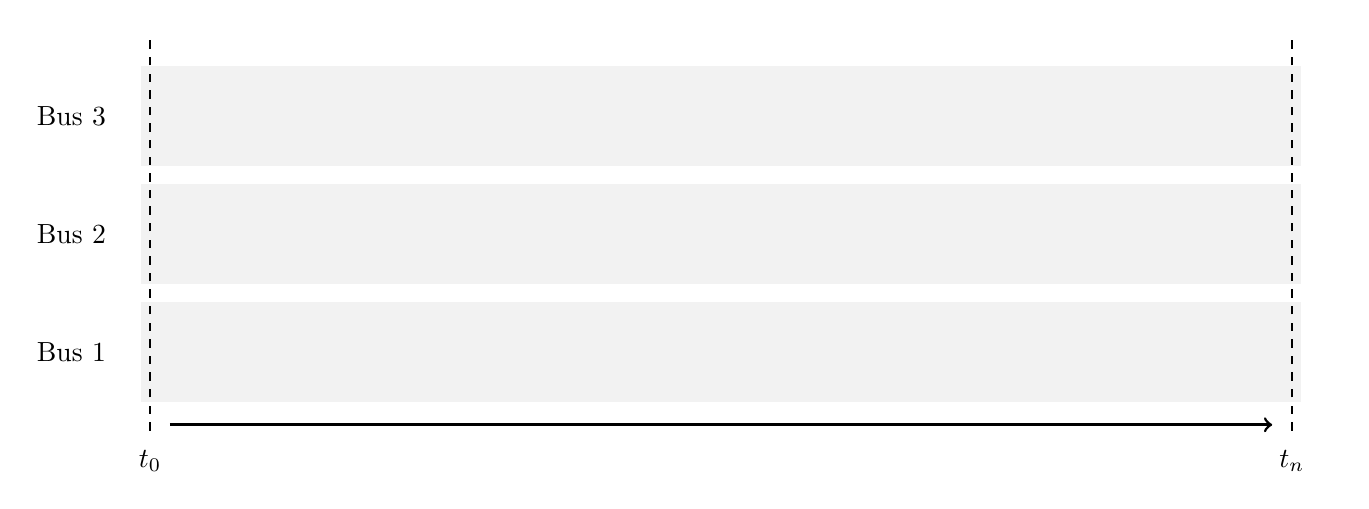
\begin{tikzpicture}
	\node[rectangle, fill=gray!10, minimum width=5.8in, minimum height=0.5in](bus1Box) at (7.75,1){};
	\node(bus1BoxLabel) at (-0.5, 1){Bus 1}; 

	\node[rectangle, fill=gray!10, minimum width=5.8in, minimum height=0.5in](bus2Box) at (7.75,2.5){};
	\node(bus1BoxLabel) at (-0.5, 2.5){Bus 2};

	\node[rectangle, fill=gray!10, minimum width=5.8in, minimum height=0.5in](bus3Box) at (7.75,4){};
	\node(bus1BoxLabel) at (-0.5, 4){Bus 3};

	\node[label=below:$t_0$](origin) at (0.5,0){};
	\node(yAxes) at (15.5,0){};
	\node(xAxes) at (0.5,5){};
	\node[label=below:$t_n$](bottomRight) at (15,0){};
	\node(topRight) at (15,5){};
	\draw[dashed, line width=0.5pt] (origin.center) -- (xAxes.center); 
	\draw[dashed, line width=0.5pt] (bottomRight.center) -- (topRight.center);
	\node(t0) at (0.75,-0.05){};
	\node(tn) at (14.75,-0.05){};
	\draw[->, line width=1pt] (t0.north) -- (tn.north); 
\end{tikzpicture}
	\caption{Description of the bus and time axis}
	\label{fig:busTime1}
\end{figure*}

\par Each bus follows a schedule made up of a series of arrival and departure times, where the bus's $n^{\text{th}}$ stop begins at arrival time $a_n$ and terminates at departure time $d_n$ (see Fig. \ref{fig:busTime3}). 
\par A bus can be assigned to charge anytime the bus is in the station. The charge start time during the $n^{\text{th}}$ stop is denoted $c_n$ and the stop-charge time is denoted $s_n$ as shown in Fig. \ref{fig:busTime3}. 
\begin{figure*}
\centering
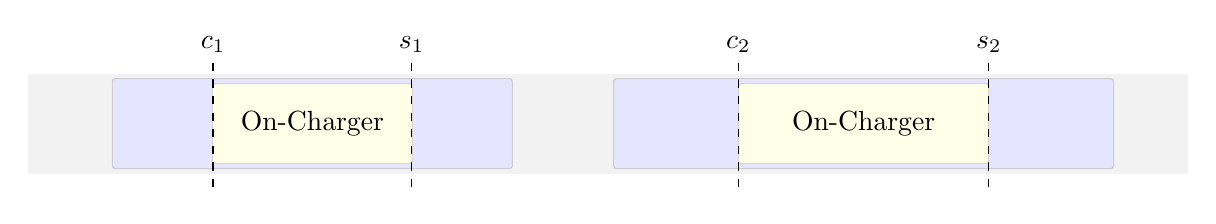
\begin{tikzpicture} 
	\node[rectangle, fill=gray!10, minimum width=5.8in, minimum height=0.5in](busSched) at (7.75,1){}; 

	\node[rectangle, draw=blue!10!black!20, fill=blue!10, minimum width=2in, minimum height=0.45in, rounded corners=1pt](busAvail1) at (4,1){In-Station};
	\node[rectangle, draw=blue!10!black!20, fill=blue!10, minimum width=2.5in, minimum height=0.45in, rounded corners=1pt](busAvail2) at (11,1){In-Station};

	\node[rectangle, draw=yellow!10!black!20, fill=yellow!10, minimum width=1in, minimum height=0.4in, rounded corners=1pt](busAvail1) at (4,1){On-Charger};
	\node[rectangle, draw=yellow!10!black!20, fill=yellow!10, minimum width=1.25in, minimum height=0.4in, rounded corners=1pt](busAvail2) at (11,1){On-Charger};


	\node(firstATop) at (2.74,2){$c_1$};
	\node(firstABtm) at (2.74,0.2){};
	\draw[dashed, line width=0.5pt](firstATop) -- (firstABtm.center);
	\node(firstDTop) at (5.26,2){$s_1$};
	\node(firstDBtm) at (5.26,0.2){};
	\draw[dashed, line width=0.5pt](firstDTop) -- (firstDBtm.center);

	\node(secondATop) at (9.41,2){$c_2$};
	\node(secondABtm) at (9.41,0.2){};
	\draw[dashed, line width=0.5pt](secondATop) -- (secondABtm.center);
	\node(secondDTop) at (12.59,2){$s_2$};
	\node(secondDBtm) at (12.59,0.2){};
	\draw[dashed, line width=0.5pt](secondDTop) -- (secondDBtm.center);


\end{tikzpicture}
\caption{Bus Charging}
\label{fig:busTime3}
\end{figure*}

\subsection{Constraints}
The relationship between the arrival, departure, and charge intervals for the $i^{\text{th}}$ bus at the $j^{\text{th}}$ stop can be expressed as a set of inequality constraints such that
\begin{equation}\begin{aligned}
	a_{ij} &< c_{ij} \\
	c_{ij} &< s_{ij} \\
	s_{ij} &< d_{ij}
\end{aligned}\end{equation}
Which can be expressed in standard form as
\begin{equation}\begin{aligned}
	-c_{ij} &< -a_{ij}\\
	c_{ij} - s_{ij} &< 0\\
	s_{ij} &< d_{ij}
\end{aligned}\end{equation}
and finally, 
\begin{equation}\label{eqn:timeConstraint}
	\begin{bmatrix} -1 & 0 \\
	                 1 & -1 \\
		0 & 1\end{bmatrix} \begin{bmatrix} c_{ij} \\ s_{ij}\end{bmatrix} \le \begin{bmatrix}-a_{ij} \\ 0 \\ d_{ij} \end{bmatrix}.
\end{equation}
	Equation \ref{eqn:timeConstraint} can be expressed in terms of $\mathbf{y}$ such that
\begin{equation} \begin{aligned}
	\begin{bmatrix}-1_c & 0 & \hdots & 0    \\
                        1_c & 0 & \hdots & -1_d \\
		0   & 0 & \hdots & 1_d \end{bmatrix}\mathbf{y} &\le \begin{bmatrix} -a \\ 0 \\ d\end{bmatrix} \ \forall i,j \\
			A_1\mathbf{y} &\le \mathbf{b}_1,
\end{aligned} \end{equation}
	where $A_1$ and $\mathbf{b}_1$ stack the constraints given in equation \ref{eqn:timeConstraint} for all $i,j$.
\par A charge plan can be formulated by reserving time slots at chargers when buses need to charge (see Fig. \ref{fig:busTime4}).
\begin{figure*}
	\centering
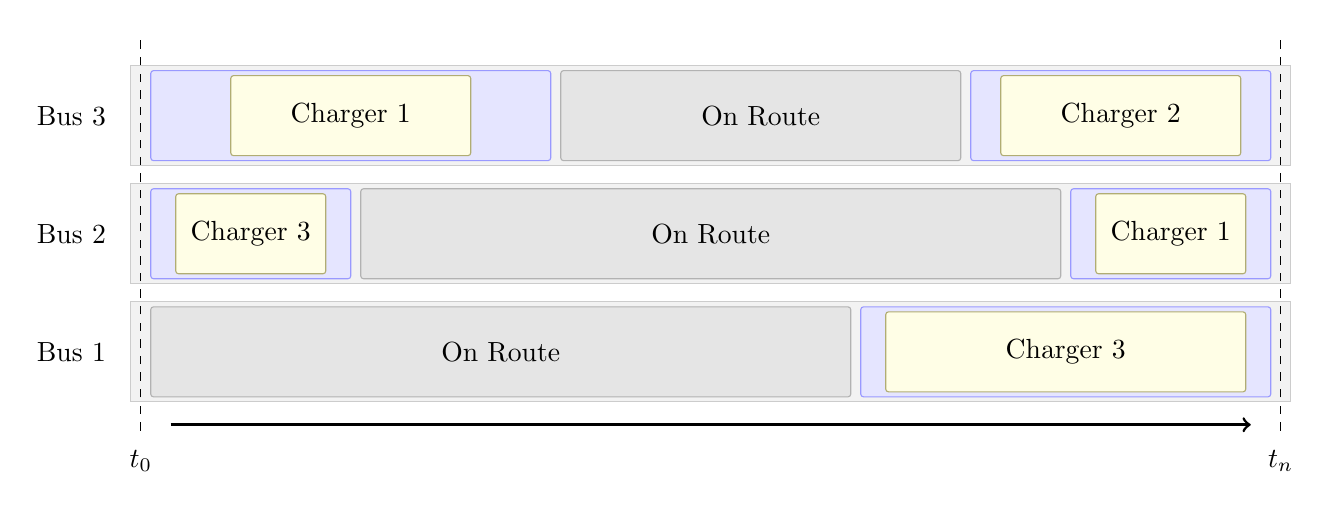
\begin{tikzpicture}
	\node[rectangle, draw=gray!40, fill=gray!10, minimum width=5.8in, minimum height=0.5in](charger1Box) at (3in,1){};
	\node(bus1BoxLabel) at (-0.5, 1){Bus 1}; 

	\node[rectangle, draw=gray!40, fill=gray!10, minimum width=5.8in, minimum height=0.5in](charger2Box) at (3in,2.5){};
	\node(bus1BoxLabel) at (-0.5, 2.5){Bus 2};

	\node[rectangle, draw=gray!40, fill=gray!10, minimum width=5.8in, minimum height=0.5in](charger3Box) at (3in,4){};
	\node(bus1BoxLabel) at (-0.5, 4){Bus 3};

	\node[label=below:$t_0$](origin) at (0.15in,0){};
	\node(xAxes) at (0.15in,5){};
	\node[label=below:$t_n$](bottomRight) at (5.85in,0){};
	\node(topRight) at (5.85in,5){};
	\draw[dashed, line width=0.5pt] (origin.center) -- (xAxes.center); 
	\draw[dashed, line width=0.5pt] (bottomRight.center) -- (topRight.center);
	\node(t0) at (0.3in,-0.05){};
	\node(tn) at (5.7in,-0.05){};
	\draw[->, line width=1pt] (t0.north) -- (tn.north); 

	% draw bus 3 boxes
	\node[rectangle, draw=blue!40, fill=blue!10, minimum width=2in, minimum height=0.45in, rounded corners=1pt](bus1Avail1) at (1.2in,4){};
	\node[rectangle, draw=yellow!50!black!70, fill=yellow!10, minimum width=1.2in, minimum height=0.4in, rounded corners=1pt](bus1Time1) at (1.2in,4){Charger 1};

	\node[rectangle, draw=black!30, fill=black!10, minimum width=2in, minimum height=0.45in, rounded corners=1pt](bus2Time1) at (3.25in,4){On Route};

	\node[rectangle, draw=blue!40, fill=blue!10, minimum width=1.5in, minimum height=0.45in, rounded corners=1pt](bus1Avail1) at (5.05in,4){};
	\node[rectangle, draw=yellow!50!black!70, fill=yellow!10, minimum width=1.2in, minimum height=0.40in, rounded corners=1pt](bus3Time1) at (5.05in,4){Charger 2};

	% draw bus 2 boxes
	\node[rectangle, draw=blue!40, fill=blue!10, minimum width=1in, minimum height=0.45in, rounded corners=1pt](bus1Avail1) at (0.7in,2.5){};
	\node[rectangle, draw=yellow!50!black!70, fill=yellow!10, minimum width=0.75in, minimum height=0.4in, rounded corners=1pt](free1) at (0.7in,2.5){Charger 3};

	\node[rectangle, draw=black!30, fill=black!10, minimum width=3.5in, minimum height=0.45in, rounded corners=1pt](bus3Time2) at (3.0in,2.5){On Route};

	\node[rectangle, draw=blue!40, fill=blue!10, minimum width=1.0in, minimum height=0.45in, rounded corners=1pt](bus1Avail1) at (5.3in,2.5){};
	\node[rectangle, draw=yellow!50!black!70, fill=yellow!10, minimum width=0.75in, minimum height=0.4in, rounded corners=1pt](free2) at (5.3in,2.5){Charger 1};

	% draw bus 1 boxes 
	\node[rectangle, draw=black!30!, fill=black!10, minimum width=3.5in, minimum height=0.45in, rounded corners=1pt](bus3Time2) at (1.95in,1){On Route}; 

	\node[rectangle, draw=blue!40, fill=blue!10, minimum width=2.05in, minimum height=0.45in, rounded corners=1pt](bus1Avail1) at (4.775in,1){};
	\node[rectangle, draw=yellow!50!black!70, fill=yellow!10, minimum width=1.8in, minimum height=0.4in, rounded corners=1pt](bus1Time2) at (4.775in,1){Charger 3};
\end{tikzpicture}
	\caption{Reserving time slots on chargers}
	\label{fig:busTime4}
\end{figure*}

	Note how there are several decisions that go into the charge schedule, namely when and to which charger a bus will connect. 
\par The variables for time have already been discussed in equation \ref{eqn:timeConstraint}, but variables for which charger have not been given.  Let $\sigma_{ijk}$ be a binary variable that is $1$ when bus $i$ charges during the $j^{\text{th}}$ stop at charger $k$. Because a bus can only charge at one charger at a time, we also constrain $\sigma$ such that
\begin{equation}
	\begin{aligned}
		\sum_k \sigma_{ijk} \le 1 \ \forall i,j
	\end{aligned}
\end{equation} 
or in standard form as 
\begin{equation} \begin{aligned}
	\begin{bmatrix}1_{ij1} & 0 & \hdots & 0 & 1_{ijk} \end{bmatrix} \mathbf{y} &\le \mathbf{1} \ \forall i,j\\
		A_2\mathbf{y} & \le \mathbf{b}_2.
\end{aligned} \end{equation}
	The variable $\sigma_{ijk}$ is used in several scenarios. The first is to constrain a zero-second charge time when not in use.  This is done as
	\begin{equation}\begin{aligned}
		s_{ij} - c_{ij} &\le M\sum_{k}\sigma_{ijk} \\
		s_{ij} - c_{ij} - \sum_{k}\sigma_{ijk}M &\le 0\\
		\begin{bmatrix} 1_s & -1_c & -M_{\sigma} \end{bmatrix}\begin{bmatrix}s_{ij} \\ c_{ij} \\ \sigma_{ij1} \\ \vdots \\ \sigma_{ijk} \end{bmatrix} &\le 0 \ \forall i,j \\
			A_3\mathbf{y} &\le \mathbf{b}_3 \\
	\end{aligned} \end{equation}
The variable $\sigma_{ijk}$ is also necessary to eliminate situations where more then one bus is assigned to a charger at the same time. Note that this can only happen when $a_{ij}$ for bus $i$ is less than $d_{i^{'}j^{'}}$ for bus $i^{'}$ as shown in Fig. \ref{fig:potentialOverlap}. Charging overlap can be avoided by constraining
\begin{figure}[ht!]
	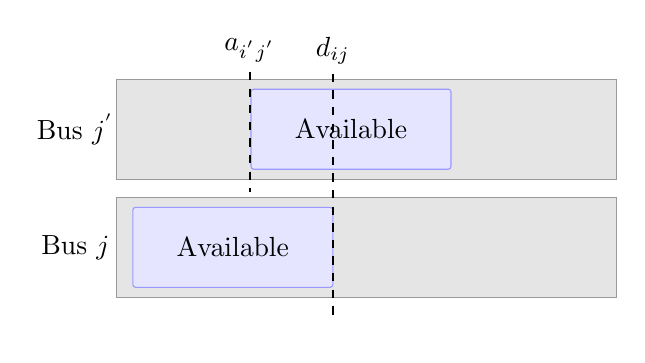
\begin{tikzpicture} 
		\node[rectangle, draw=black!40, fill=black!10, minimum width=2.5in, minimum height=0.5in](charger1Box) at (3.2,1){};
		\node(bus1BoxLabel) at (-0.5, 1){Bus $j$}; 
		\node[rectangle, draw=black!40, fill=black!10, minimum width=2.5in, minimum height=0.5in](charger2Box) at (3.2,2.5){};
		\node(bus1BoxLabel) at (-0.5, 2.5){Bus $j^{'}$};
		\node[rectangle, draw=blue!40, fill=blue!10, minimum width=1in, minimum height=0.4in, rounded corners=1pt] at (1.5,1){Available};
		\node[rectangle, draw=blue!40, fill=blue!10, minimum width=1in, minimum height=0.4in, rounded corners=1pt] at (3,2.5){Available};
		\node(aJPrimeHigh) at (1.72,3.5){$a_{i^{'}j^{'}}$};
		\node(aJPrimeLow) at (1.72,1.7){};
		\node(dJHigh) at (2.77,3.5){$d_{ij}$};
		\node(dJLow) at (2.77,0.0){};
		\draw[dashed, line width=0.5pt] (aJPrimeHigh) -- (aJPrimeLow.center);
		\draw[dashed, line width=0.5pt] (dJHigh) -- (dJLow);
	\end{tikzpicture}
	\caption{Potential Overlap}
	\label{fig:potentialOverlap}
\end{figure}



\begin{align}\label{eqn:overlapConstraints1}
c_{i^{'}j^{'}} > s_{ij}.
\end{align}
However, this constraint is only necessary when both bus stops are designated for charging. This can be remedied as
	\begin{align}\label{eqn:overlapConstraints2}
		c_{i^{'}j^{'}} - s_{ij} > M\left[(\sigma_{i^{'}j^{'}k} + \sigma_{ijk}) - 2\right] \ \forall k
	\end{align}
	Where $M = 2\cdot\text{nTime}$. When $(\sigma_{i^{'}j^{'}k} + \sigma_{ijk}) < 2$, equation \ref{eqn:overlapConstraints2} is trivially satisfied for all values of $c_{i^{'}j^{'}}$ and $s_{ij}$. When $\sigma_{i^{'}j^{'}k} = \sigma_{ijk} = 1$, equation \ref{eqn:overlapConstraints2} simplifies to equation \ref{eqn:overlapConstraints1}. Equation \ref{eqn:overlapConstraints2} can be expressed in standard form as 
	\begin{equation}\label{eqn:overlapConstraints3}\begin{aligned}
		-c_{i^{'}j^{'}} + s_{ij} + M\sigma_{i^{'}j^{'}k} + M\sigma_{ijk} &\le 2M  \ \forall k\\
	\end{aligned}\end{equation}
	and finally as
	\begin{equation}\begin{aligned} 
		\begin{bmatrix} -1 & 1 & M & M\end{bmatrix} \begin{bmatrix}c_{i^{'}j^{'}}\\ s_{ij} \\ \sigma_{i^{'}j^{'}k}\\ \sigma_{ijk} \end{bmatrix} &\le 2M \ \forall k
	\end{aligned} \end{equation}
	The constraints in equation \ref{eqn:overlapConstraints3} can be repeated for all instances where overlap is possible and concatenated into a single matrix such that
	\begin{equation}\begin{aligned} 
		A_4\mathbf{y} & \le \mathbf{1}\cdot 2M \\
		A_4\mathbf{y} & \le \mathbf{b}_4 \\
	\end{aligned} \end{equation} 
